\documentclass[12pt,a4paper]{article}
% vim: set textwidth=100:

\usepackage{amsmath}
\usepackage{amsfonts}
\usepackage{amsthm}
\usepackage{hyperref}
\usepackage[pdftex]{graphicx}

\title{Associative Data Structures for Website Filtering}
\author{Jelco Bodewes, Pieter Brederode \\ Anton Golov, Timo Koppenberg }

\begin{document}
    \maketitle

    \begin{abstract}
        We have researched the performance of the hash table, binary search tree, and skip list
        associative datastructures in the context of a web filter.  Our measurements were made with
        structures of various sizes (ranging from $2^8$ up to $2^{20}$) and with different possible
        key types (from 4 to 120 bytes).  In this paper, we describe our implementation and
        empirically show that given a sufficiently high number of entries, a hash table has the
        highest insertion and query speeds, while the skip list requires the least memory per
        element.
        % And when I say "hash table", I mean libstdc++'s unordered_map, and when I say bst I mean
        % libstdc++'s map, and if you took different implementations you'd probably get different
        % results...
    \end{abstract}


    \section{Introduction}
    A website filter is a program that categorises websites in order to restrict access to
    designated sites a user might visit. Commonly, the filter operates by keeping a blacklist of
    sites a user may not visit unless they have certain credentials, or alternatively, keeping a
    whitelist and prohibiting any sites not on it.  As the world-wide web is growing, these lists
    have grown larger to a point where the speed of the underlying data structure has become a key
    issue.  The time of both inserting and looking up websites must be kept minimal. Moreover, the
    increased number of entries make memory usage an equally significant concern.

    In technical terms, we are interested in the best data structure for associating many URLs with
    their respective permissions, be it whitelisted or blacklisted for certain users.  We have
    chosen to compare the performance of the binary search tree, the hash map, and the skip list, as
    these are commonly employed in practice.  It is of particular interest how each data structure
    will scale as the number of elements rises.  We have thus chosen for our main research question
    the following:
    % Guys, did you notice we did absolutely nothing about predicting this?

    \begin{quotation}
        How does the number of entries influence the performance of various associative data
        structures?
    \end{quotation}

    While the decision of data structure might mostly be dependant on the number of entries, the
    complexity of the key might also be of concern. Where permissions per page would be preferred, a
    more resource optimal solution might be found in filtering only on domain or even IP adress.  In
    researching the influence of this we formulate a secondary research question:

    \begin{quotation}
        How does the complexity of the key influence the preformance of various associative data structures?
    \end{quotation}

    In this paper, we attempt to answer these questions. Section~\ref{sec:plan} provides details
    about our research plan and the scopes of our research. Section~\ref{sec:implementation} is
    about the implementation of our setup in C++.  The rest of the paper states our results and the
    conclusions that can be drawn from them.

    \section{Research Plan}
    \label{sec:plan}

    \subsubsection*{Scope and assumptions}

    We make several assumptions for our research.

    Firstly we plan on only working with datasets that are certain to fit into the main memory of our machine. We intend to
    purely examine the relative speed and memory-efficiency of the different data structures. Using datasets larger than
    memory will cause regular lookups to the harddrive, which we assume would skew our results.

    In order to make the measurements more predictable, we will always ensure that insertions are only performed with
    non-existent keys. The alternative would make either the memory usage or number of insertions non-deterministic, which
    could cause inaccuracies in measurement. Similarly, we require that all queries be performed on existing keys.

    To mimic real usage, we will insert and then access the keys in an arbitrary order.  However, we will keep the order consistent
    between tests on different data structures.  Together this will minimize any bias related to any kind of order-dependent
    performance, which would likely be an advantage specific to the implementation, not to the data structure. We will
    generate the order for both lookup and insertion by shuffling the dataset we chose for the specific test. This means that
    orders will not be persistent between different data set sizes; however, we do not expect this to be significant.

    We realize that methods to measure the amount of time required for actions will themselves need time. We will however
    use the same time-measuring method for all data structures, so we can still use the results to compare the different
    data structures.

    \section{Implementation}
    \label{sec:implementation}

    We used C++ implementations of the data structures involved, and also the language for our
    measuring code.  We chose C++ as it is an industry standard\footnote{ref}, provides the
    necessary tools, and does not carry the risk of garbage collection pauses or effects due to
    ``warming-up time''.

    \subsection*{Data Structures}

    Using C++ as the implementation language, we chose libstdc++'s implementations of the standard class
    templates \texttt{std::map} and \texttt{std::unordered\_map} for the binary search
    tree and the hash table respectively.  As the C++ standard library does not contain a skip
    list\footnote{reference to the standard here}, we used an open-source third party library,
    \texttt{CSSkipList}\footnote{reference to library home page here}.  We also used libstdc++'s
    implementation of \texttt{std::string} for our string handling\footnote{specify?}needs.

    \subsubsection*{Data}
    For our data, we used datasets containing $2^x$ elements with $x$ an integer such that $8 < x <
    21$. Thus we have twelve different dataset sizes. We took the system's dictionary file and the
    list of top level domains from Wikipedia and combined these to generate a list of items in the
    form \texttt{www.\$word.\$tld}, where \texttt{\$word} is one of words from the the dictionary
    and \texttt{\$tld} is a top level domain.  Only words consisting of the lowercase letters
    \texttt{a} through \texttt{z} were used. Constraining the words to consist of 8 to 12 characters
    and limiting the top-level domains to exactly two letters, all possible combinations were
    generated.  For the full paths, a number of domains were selected and each was appended a random
    alphanumeric string of eighty characters.  Finally, for the third type of key, an IP address, we
    used 32 bit integers. The exact implementation can be viewed in the sourcecode\footnote{ref to
    apendix or code dump}.

    \subsection*{Measurements}
    For our time measurements, we used libstdc++'s implementation of the standard
    \texttt{std::chrono::high\_resolution\_clock} class.

    Memory measurements were performed by providing a custom allocator which tracked the number of
    memory requests.  Note that the latter deviates from our initial plan, where we
    stated\footnote{ref?}we would use the POSIX API\footnote{ref to the posix api}.  Unfortunately,
    that turned out to be too coarse-grained for our purposes and we could thus get no accurate
    measurements.  The allocator-based technique we employed did require some slight modifications
    to the skip list implementation we used, but this should not have caused a significant slowdown.
    We assume that any influence will only have made the tests more fair, as now allocation was done
    the same way in all three setups.

    After some tests we chose to decrease the number of runs used for measurements.  In the proposal
    we stated that for each time measurement we would perform the relevant operation 1000 times and
    then take the average of that.  In practice, this made the tests run for longer than we could
    afford. Because the results given by performing 100 runs were comparable, we settled for that.
    We expect the general result to be similar; refer to section\footnote{ref}for details about what
    \emph{could} have gone wrong.

    \section{Results}

    Now that we have done the tests we have gained a lot of data that we can analyze and base our 
    conclusions on. To do this, we will need to make our data more easily readable and use statistical
    tests to draw conclusions.

     First, to get an overview of our data, we will determine the averages for each scenario
    (Datastructure, keytype and number of entries). For these averages we will look at operation speed per
    element and memory usage per element. These can be seen in appendix \ref{App:AveResults}.

    Now we may notice patterns in these averages, but to actually draw conclusions from the results, we will
    need to use statistical methods. Depending on what results we want to compare there are different statistical
    tests we can use. For our results we shall make use of independent samples T test and bivariate correlation test.

    We shall use a significance of $0.95$ and we perform all statistical tests using the SPSS software package.

    \subsection{Correlation between number of entries and results}
    First we look at the influence the number of entries has on the per element speed of operations. For this
    we will use a bivariate correlation test, since we want to check if there exists a correlation between 
    the number of entries and the speed of operations.

    Using analysis in SPSS it turns out that for almost all situations there exists positive correlations between the number
    of entries and the speed of both queries and inserts. For both skiplist and BST these correlations are significant for all
    keytypes. In all cases they have positive correlations between $0.4$ and $0.6$. 

    However in the case of hashmaps we don't always have correlations. For all situations there does exist a positive correlation
    between the number of entries and the per element query time. But for inserts there only exists a correlation when we 
    look at Ip-address keys. If we look at Domain or Full path keys, there is no significant correlation between the number of entries
    and the per element speed of insert operation. 

    \subsection{Difference in performance between different keytypes}
    Another part of our research question was: ``How does the complexity of the key influence the performance of 
    various associative data structures?". Thus we would like to compare performance between the different keytypes. 
    To look at this, we will set our number of entries to 4096 and compare the different key types.

    It turns out the results are largely the same for the different data structures. For all of the data structures the use of
    Ip-addresses is significantly faster in both query and insert speeds and has lower memory usage as well, this is even true
    no matter the number of entries. 

    For the difference between full path and domain the results become more complex. Looking at BST we get the following results:
    Insert speed on full paths is significantly faster than insert speed on domains, however query speed on domains is significantly faster
    than query speed on full paths. 

    Looking at skiplist we get the following results: Insert speed on full paths is significantly faster than insert speed on domains. Query
    speed however does not significantly differ between domains and full paths. If we look at higher number of entries query speed becomes 
    significantly faster for full paths. 

    Finally for our results with hashmap: Domains are significantly faster in both insert and query speed compared to full paths. 
    This is true no matter the number of entries.

    \subsection{Comparison between different data structures}
    We would like to be able to use our results to determine which data structures are better in which cases. 
    For this we will have to compare the different data structures for specific situations. We will use an independent
    samples T test for this, since our data points are independent of each other. 

    First off, for almost all situations with the keytypes Full path and Domain, hashmap is significantly faster than BST and skiplist
    in both query speed and in insert speed. The only exception is in the case of 256 entries, which is most likely a
    problem in our setup. 

    More interesting are the speeds in the case of the Ip-addresses. While the hashmap is still significantly faster 
    for query speeds, no matter the number of entries, there is a different result for the insert speeds. For 4096
    entries or less, the BST significantly outperforms the hashmap in terms of insert speed. For any number of 
    entries higher than that, the hashmap outperforms the BST again. 

    
    

    \subsection{Errors possibly caused by an imperfect implementation}

    There were a number of measurements that did not follow the underlying theory and are likely a
    consequence of the hardware involved.

    In particular, constructing a small hash table\footnote{state the number of elements in a
    "small" hash table} after constructing many big ones takes a disproportionally long time.  Only
    the first hash table is affected, and the time is comparable to the time required to construct a
    hash table with 4000 elements, which is illogical.  We assume this is caused by the allocator
    but the reason for such behaviour is still unclear.  The fact that a hashtable needs contiguous
    memory is likely to have some influence, as well as the allocator returning memory to the
    operating system.  However, we reason the latter should also have happened with the other
    structures.

    A similar issue occurs around 4000 or 8000 elements (depending on data structure).  For all
    three datastructures, the cost of inserting and querying grows at a higher rate than before.
    This is difficult to quantify\footnote{Can we do some sort of linear regression to prove this is
    the case?}, but it appears some extra load is added at that point.  We suspect it is related
    either to the allocator having to acquire more memory or the CPU cache running out and more
    cache misses occuring.  We would measure this as well, if there was more time.

    A potentially related issue is that the standard deviation of our measurements rises around the
    same point.  That increases the likelihood of it being allocator-related, as that involves a
    system call and could cause scheduling issues\footnote{elaborate/ref?}, despite the system being
    otherwise very close to idle.

    Also, we acquired counterintuitive results showing that inserting or querying a full path is
    faster than querying only the domain name.  This can partially be explained\footnote{Not really,
    but ehhh.}by the fact that the string implementation we used was based on reference counting.
    %(If it'd also provide SSO, this would be easy to explain, but the darn thing doesn't.)

    \section{Conclusions}
    Our main point of research was researching which associative data structure performed best on a
    various number of insertions, in terms of the speed of insertions and look-ups, and memory
    usage.  In terms of speed we can state with certainty that the hash table is the superior data
    structure.  It outperforms the other two in almost every category, most significantly in larger
    datastructures where it often takes less than half as much time as the skiplist and less than
    two thirds the time of the binary search tree.  In most cases, the binary search tree is a bit
    slower, whereas the skip list is the slowest structure in virtually every case. The only
    motivation for using a skiplist for this problem appears to be in memory usage, although the
    advantage gained from this is relatively small.

    Our secondary point of research encompassed the effect of key complexity on associative data
    structures.  Our different types of keys were IP adresses, domain names and full path URLs. We
    have seen that as expected, IP adresses as keys provide a significant improvement over the other
    two, and uses less memory as well. Interesting to note is that we found the only advantage of
    the binary search tree over the hashmap here, is that insertions of a small amount of IP
    adresses, up to around $2^13$ insertions, is faster. So when writing an application with very
    few keys of low complexity, and with more insertions than queries, the binary search tree may be
    the best option. Finally, we have found that the domain key type does not outperform the full
    path key type. It is not significantly better if it is better at all.

    \section{Reflection}
    In general, we are content with the results of our research. We were able to provide clear and
    concise answers to our research questions. Even though our research questions may appear broad,
    we have defined a good scope in our research proposal and have virtually not altered this scope
    in our research. One small change is that we also included datasets of size $2^8$ because we saw
    some interesting results in very small sets. In our implementation we have made some significant
    changes because we ran into pratical problems. Some of these required us to change the allocator
    and generate our keys in a slightly different fashion, which we all documented in this paper.

    Since we have found that the hash map is the best associative data structure overal for this
    problem, we could do further research in different kind of hash maps. We might try different
    hash functions, different methods of collision resolution, and perhaps survey different kinds of
    concurrent hash maps.

    \bibliographystyle{alpha}

    \bibliography{paper}

    \newpage
    \appendix
    \section{Average results} \label{App:AveResults}

    \begin{figure}[h!]
    \centering
    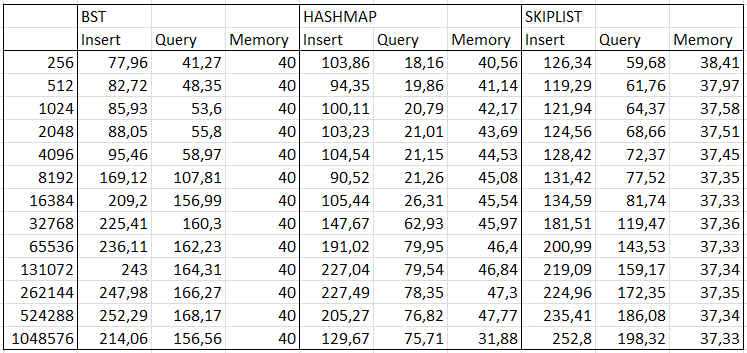
\includegraphics[width=\textwidth]{Ip-address_averages.png}
    \caption{The average per element results for each situation with Ip-adresses.}
    \end{figure}

    \begin{figure}[h!]
    \centering
    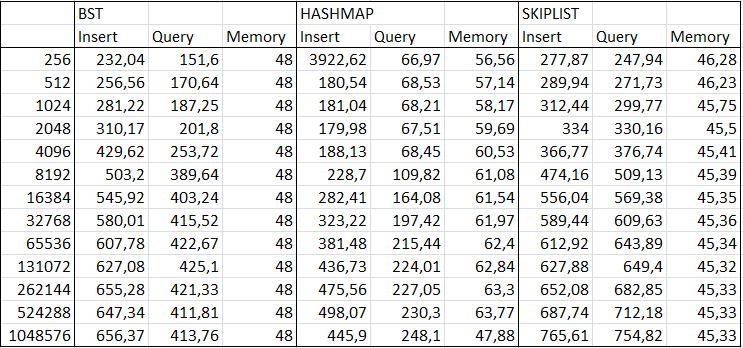
\includegraphics[width=\textwidth]{Domain_averages.png}
    \caption{The average per element results for each situation with domain adresses.}
    \end{figure}

    \begin{figure}[h!]
    \centering
    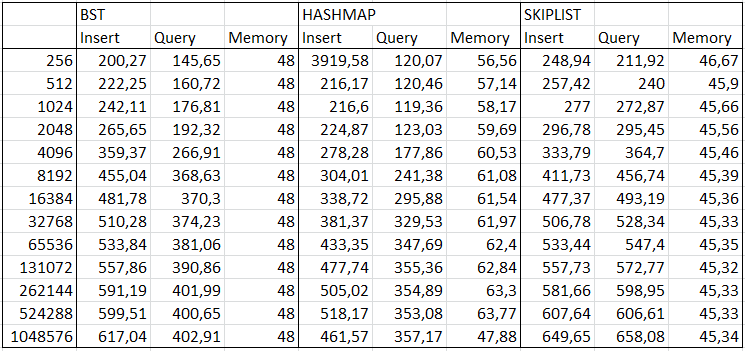
\includegraphics[width=\textwidth]{Full_path_averages.png}
    \caption{The average per element results for each situation with full path adresses.}
    \end{figure}

\end{document}
